\documentclass{beamer}

\usepackage{fourier} 
\usepackage{pifont,mdframed}
\usepackage{booktabs}
\usepackage{color, soul}
\usepackage{spot}
\definecolor{celestialblue}{rgb}{0.29, 0.59, 0.82}

\newenvironment{warning}
  {\par\begin{mdframed}[linewidth=1pt,linecolor=celestialblue]%
    \begin{list}{}{\leftmargin=1cm
                   \labelwidth=\leftmargin}\item[\Large\danger]}
               {\end{list}\end{mdframed}\par}

\newcommand{\memph}[1]{\alert{#1}}

\title{Building a Collaborative Culture \\ A Grounded Theory of Well Succeeded DevOps \\ Adoption in Practice}

\author{Welder Pinheiro Luz \textsuperscript{1} \and Gustavo Pinto \textsuperscript{2} \and Rodrigo Bonif\'{a}cio \textsuperscript{3}}

\institute{\textsuperscript{1} Brazilian Court of Accounts \and \textsuperscript{2} Faculty of Computing, Federal University of Par\'{a} \and \textsuperscript{3}
Computer Science Department, University of Bras\'{i}lia}

\begin{document}

\begin{frame}
 \titlepage
\end{frame}

\begin{frame}

  \centering{
    \huge{research context} 
  }
\end{frame}


\begin{frame}
  \frametitle{Brazilian Federal Court of Accounts (TCU)}

  \begin{block}{Characteristics}
   \begin{itemize}
    \item a huge number of enterprise systems   
    \item prevalence of JEE architecture using a shared domain model \pause
    \item clear separation between development and production teams
    \item rigid time frames for publishing software assets (once a week)  
  \end{itemize}
  \end{block}
  
\end{frame}

\begin{frame}
  \begin{center}
    \begin{huge}
      well known problems 
    \end{huge}
  \end{center}
  \pause
  
  \begin{warning}
    Use of agile development practices\pause, though expecting delays
    when publishing the software into acceptance
    testing and production environments. 
  \end{warning}
  
\end{frame}


\begin{frame}
  \begin{center}
    \begin{huge}
      well known problems 
    \end{huge}
  \end{center}
  \pause
  
  \begin{warning}
    The program works at the development environment, but
    it does not at the acceptance testing and production environments. \pause
    ``It must be a bug of the program, so the development team must
    take care of it''.
  \end{warning}
  
\end{frame}

\begin{frame}

  Let's try fixing this issue using a {\color{blue}DevOps} approach!!!
  
\end{frame}


\begin{frame}
 \centering{
    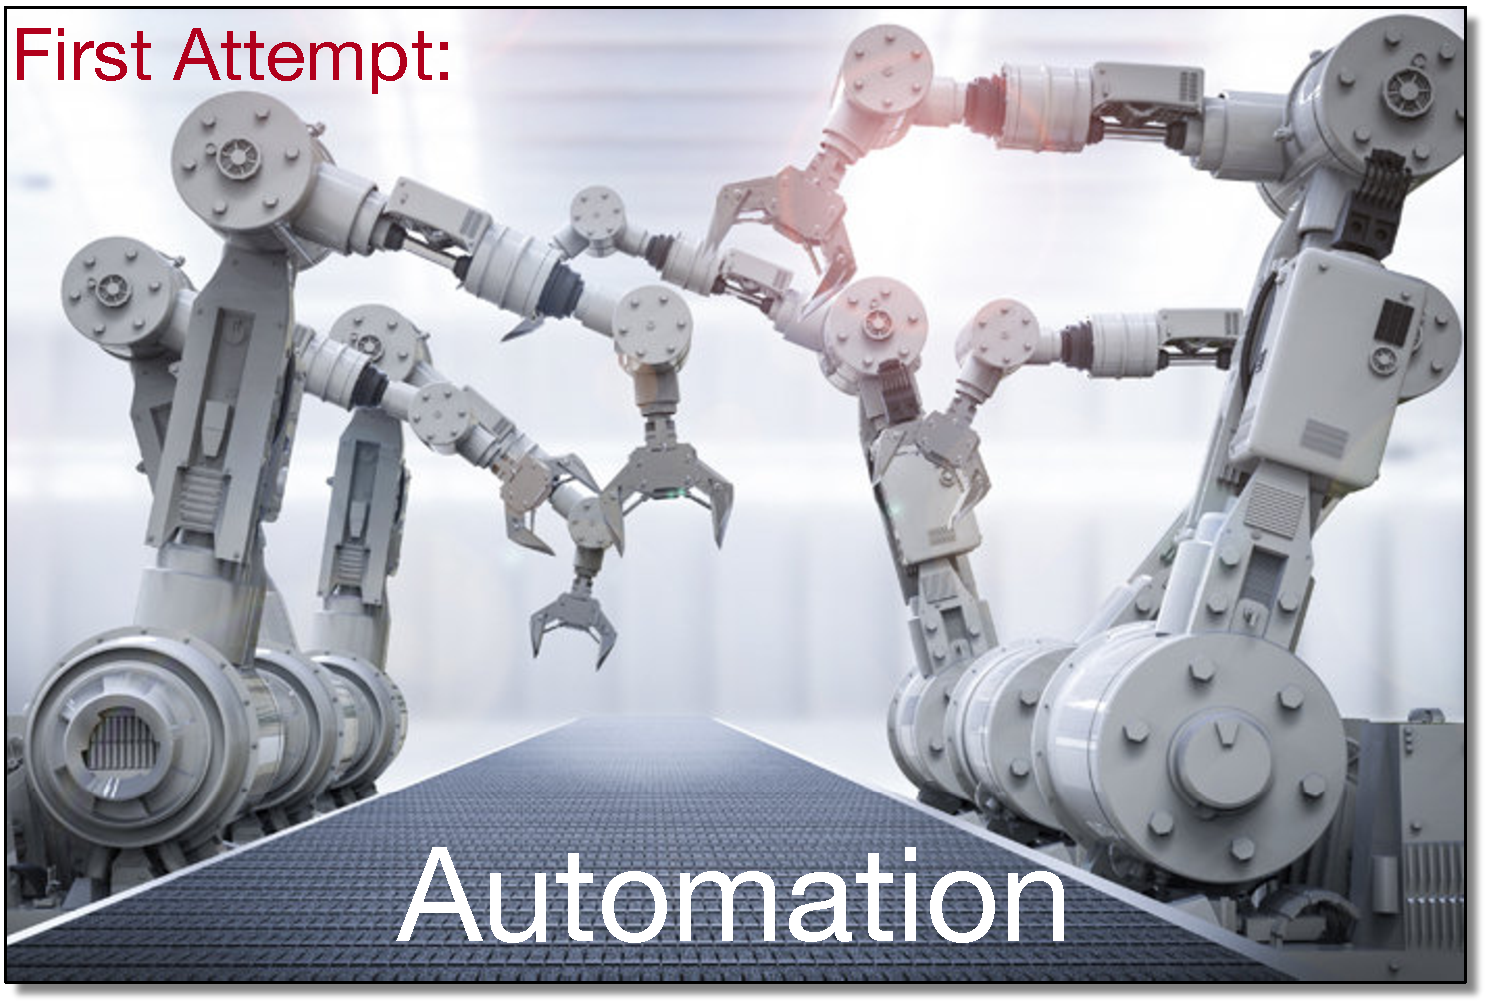
\includegraphics[scale=0.45]{images/automation}
 }
\end{frame}

\begin{frame}
  \centering{
    
\includegraphics[scale=0.5]{images/failed}
  }
\end{frame}

\begin{frame}
  \centering{
    
\includegraphics[scale=0.5]{images/research}
  }
\end{frame}

\begin{frame}

  \begin{description}
   \item[goal:] understand and characterize DevOps
   \item[method:] (classical) grounded theory approach
   \item[research question:] what are the recommendations for DevOps adoption?   
  \end{description}
\end{frame}

\begin{frame}
  \centering{
    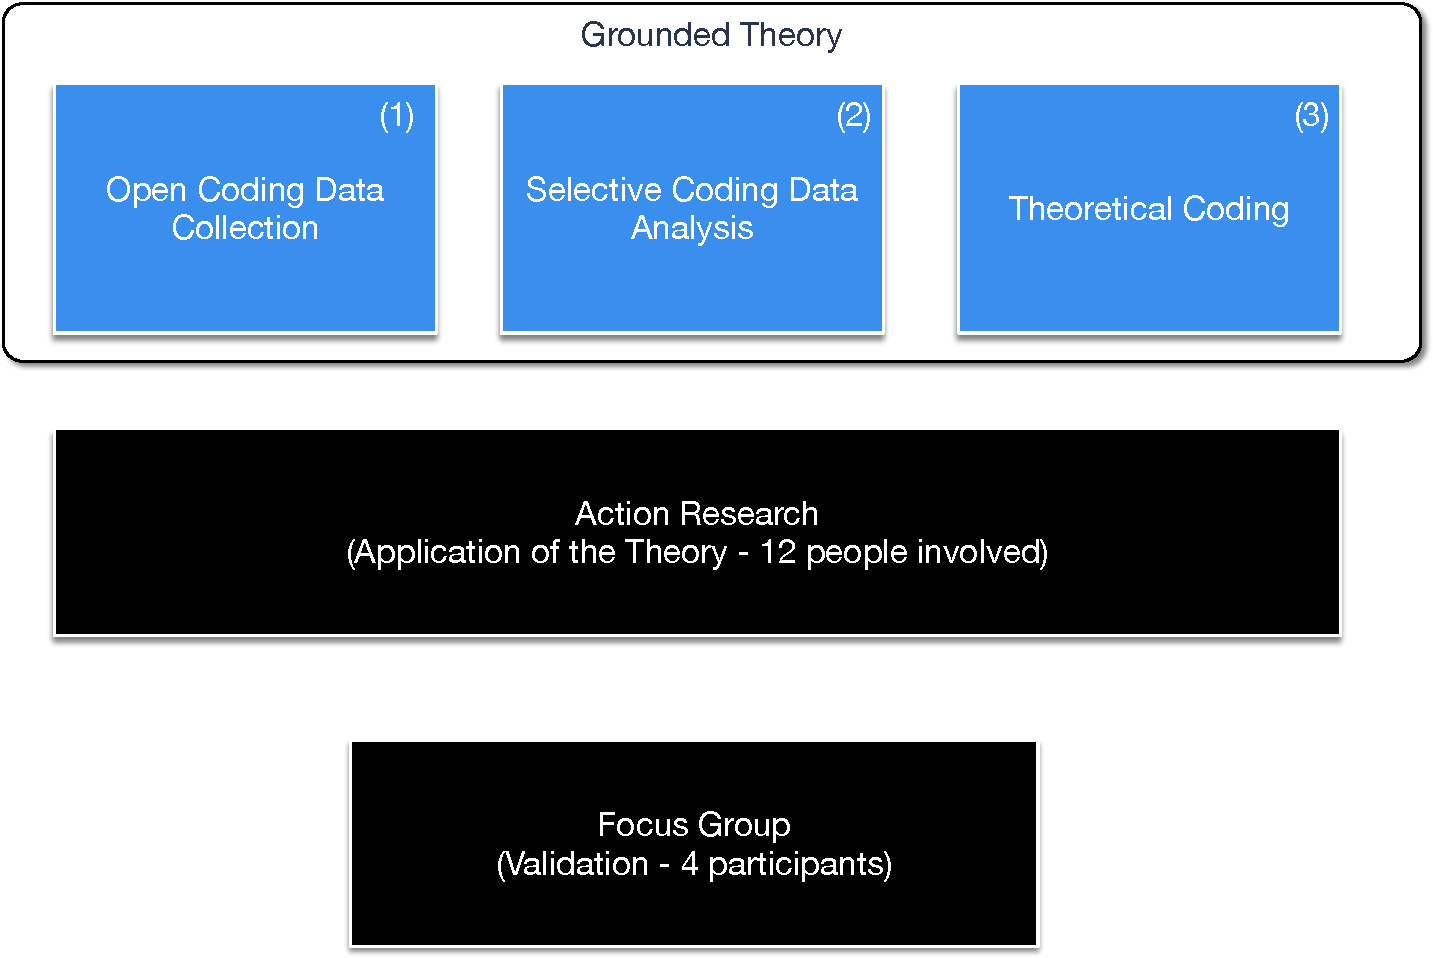
\includegraphics[scale=0.4]{images/process.pdf} 
    }
\end{frame}


\begin{frame}
\huge{Results} 
\end{frame}

\begin{frame}
  \begin{center}
    {\color{blue}Core Category}\pause
    \vskip+1.5em
    \begin{huge}Collaborative Culture\end{huge}

  \end{center} \pause
  \vskip1.5em
%  \begin{block}{Core Category:}
    \begin{itemize}
%    \item Collaborative Culture \pause
    \item Removing silos between development and production teams \pause
    \item Concepts:
      \begin{itemize}
       \item software development empowerment
       \item operations tasks should be performed by development teams \pause
       \item product thinking
       \item straightforward communication \pause
       \item blameless and shared responsibilities  
      \end{itemize}
    \end{itemize}
%  \end{block}
  
\end{frame}

\begin{frame}
  \frametitle{Not only automation}

  \begin{flushright}
    ``\emph{During a process for DevOps adoption, there is a very
    strong cultural issue that the teams sometimes are not adapted to.
    Regarding that, \memph{one thing that bothers me} a lot and that I see very often
    is \memph{people hitching DevOps exclusively by tooling or automation}.}''
  \end{flushright}
\end{frame}

\begin{frame}
  \frametitle{Product Thinking}

  \begin{flushright}
    ``\emph{We wanted to \memph{hire people who could have a product vision}.
    People who could see the problem and think of the best solution to it, 
    \memph{not only thinking of a software solution, but also the moment when that
    application will be published}. We also brought together developers to
    reinforce that everyone has to think of the product and not only in their
    code or in their infrastructure.}''
  \end{flushright}
\end{frame}

\begin{frame}
  \frametitle{Software Development Empowerment}

  \begin{flushright}
    ``\emph{It was not feasible to have so many \memph{developers} generating artifacts
    and \memph{stopping their work to wait for another completely separate team to publish it}.
    Or needing a test environment and having to wait for the operations team
    to provide it only when possible. These activities have to be available
    to quickly serve the development team.''} 
  \end{flushright}
\end{frame}

\begin{frame}
 %  \frametitle{Additional Categories}

  \begin{center}
    {\color{blue}Additional Categories}
  \end{center}\pause \vskip+1.5em
  % \begin{huge}Additional Categories\end{huge}

    \begin{block}{Enabler categories}
      \begin{itemize}
      \item automation
      \item transparency and sharing 
      \end{itemize}
    \end{block}  \pause

    \begin{block}{Categories of expected outcomes}
      \begin{itemize}
       \item agility
       \item resilience (auto-scaling and recovering) 
      \end{itemize}
    \end{block} 

\end{frame}

\begin{frame}
  
    \begin{itemize}
      \item two categories in a gray area: quality assurance and continuous measurement. 
    \end{itemize}

    
    %% \begin{small}
    %% \begin{center}
    %% \begin{tabular}{ll}\toprule
    %%   Enabler Categories & Categories of expected outcomes          \\ \midrule
    %%   automation                 & agility                          \\
    %%   transparency and sharing   & auto-scaling and recovering      \\ \bottomrule
    %%  \end{tabular}  
    %% \end{center}
    %% \end{small}
\end{frame}


\begin{frame}
  \frametitle{Collaborative Culture and Automation}

  \begin{flushright}
    When a developer needed to build a new application, the \memph{previous workflow
    demanded him to create a ticket to the operations teams}, which should then
    manually evaluate and solve the requested issue. This task could take a lot
    of time and there was no visibility between teams about what was going on\ldots.
    Today, \memph{those silos do not exist anymore within the company}, in particular because
    \memph{it is not necessary to execute all these tasks manually}. 
  \end{flushright} 
\end{frame}

\begin{frame}
  \frametitle{Knowledge Sharing}

  \begin{flushright}
    So, here we have adopted this type of strategy that is the \memph{infrastructure as code},
    consequently we have the versioning of our entire infrastructure \memph{in a common language},
    in such a way that \memph{any person}, a developer, an architect, the operations guy, or even
    the manager, \memph{can understand the settings of an application} in a particular environment.
    So, transparency aggregates too much value for us \ldots 
  \end{flushright}
\end{frame}

\begin{frame}
  \begin{center}
    {\color{blue}A Theory for DevOps Adoption}
  \end{center}\pause \vskip+1.5em
  
  \begin{center}
    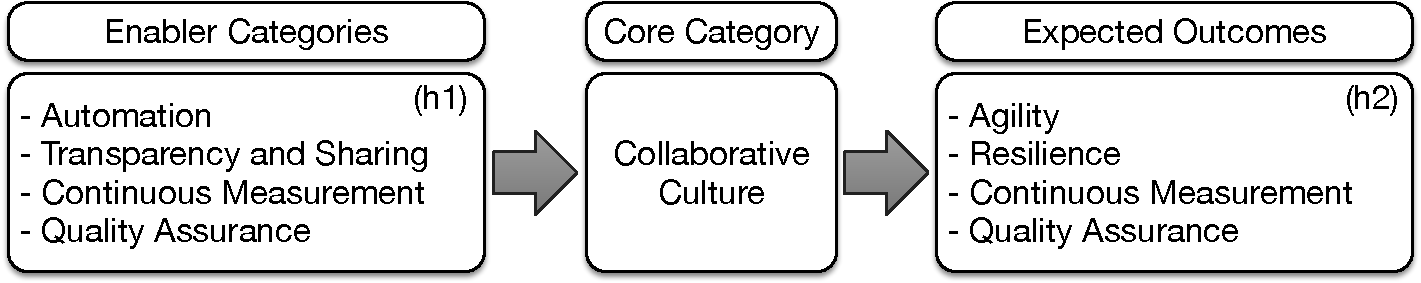
\includegraphics[scale=0.4]{images/theory.pdf}
  \end{center}
\end{frame}

\begin{frame}
  \begin{center}{\color{blue}Application at TCU}\end{center} \pause

   \begin{itemize}
     \item disseminate the needs for a collaborative culture
     \item promote tech talks and direct communication 
     \item automation and (still limmited monitoring) of several tasks
     \item infrastructure configuration as code 
    \end{itemize}
   
\end{frame}

  \begin{frame}
    \begin{center}
    \begin{tabular}{ll}\toprule
      System & Max. Number of Successful Builds in a Day \\ \midrule
      e-TCE & 29 builds \\
      e-Denuncia & 31 builds \\
      e-Representacao & 33 builds \\
      Conecta TCU & 42 builds \\
      \ldots & \\ \bottomrule
    \end{tabular}
    \end{center}

    \pause
    
    A general understanding that our model is fostering the
    adoption of DevOps practices at TCU. 

    \end{frame}
    
\begin{frame}
  \begin{center}
    {\color{blue}Challenges}
  \end{center}\pause \vskip+1.5em

  \begin{itemize}
   \item lack of a general understanding about DevOps 
   \item core ideas do not reflect the structure of TCU 
   \item limited use of monitoring services 
   \item security concerns (developers do not understand security) 
  \end{itemize}
\end{frame} 


\begin{frame}
  \begin{center}
    {\color{blue}Personal Considerations}
  \end{center}\pause \vskip+1.5em

  \begin{itemize}
  \item Does DevOps mean the death of operation teams? \pause
  \item Does DevOps practices introduce too much complexity?   
  \end{itemize}
\end{frame}

\begin{frame}
  \centering{
    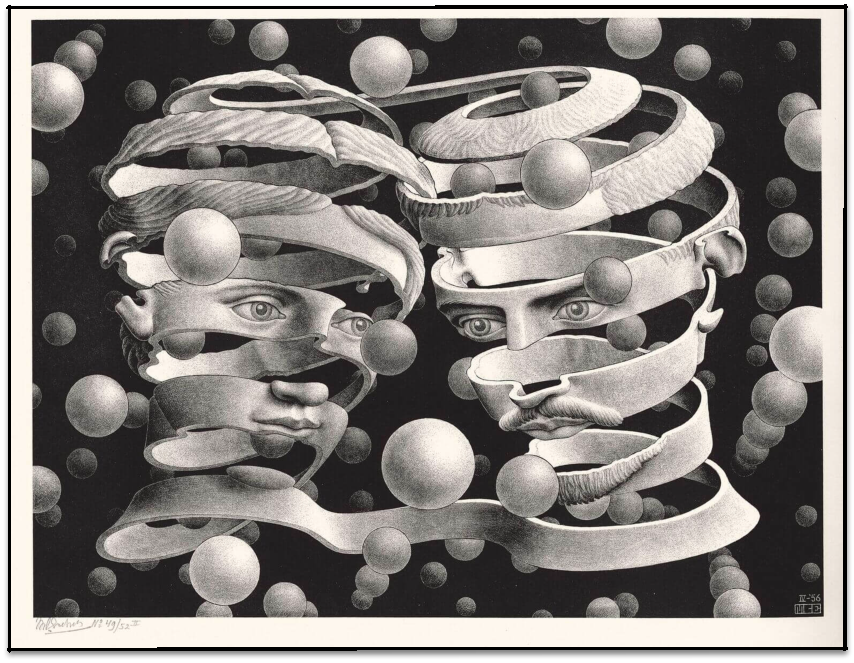
\includegraphics[scale=0.5]{images/escher.pdf}
    }
\end{frame}
\begin{frame}
\titlepage
\end{frame}


%% \begin{frame}
%%   \begin{center}
%%     
\includegraphics[scale=0.2]{images/process-01.pdf}
%%   \end{center}

  
%%   \begin{itemize}
%%     \item semi-structured interviews
%%     \item 15 participants (different countries, companies, and roles)
%%     \item goal: identify the \emph{core category}
%%   \end{itemize}
%% \end{frame}

%% \begin{frame}
%%   \begin{center}
%%     
\includegraphics[scale=0.2]{images/process-01.pdf}
%%   \end{center}


%%   \begin{block}{Core category}
%%   \begin{itemize}
%%    \item Automation (in a first moment) \pause
%%    \item Collaborative Culture (after the third interview). \pause
%%      Concepts like \emph{shared responsability} and \emph{product thinking}
%%      could not be explained around automation. \pause
%%    \item After the tenth interview, we unequivocally concluded that
%%      Collaborative Culture was the core category of our investigation.  
%%   \end{itemize}
%%   \end{block}
%% \end{frame}

%% \begin{frame}
%%   \begin{block}{(P9, IT Manager, Brazil)}
%%   \emph{In a DevOps adoption, there is a very strong cultural issue
%%   that the teams sometimes are not adapted to. Regarding that, one thing
%%   that bothers me a lot and that I see very often is people hitching DevOps
%%   exclusively by tooling or automation.}
%%   \end{block}
%% \end{frame}
    

%% \begin{frame}
%%   \begin{block}{(P5, Systems Engineer, Spain)}
%%   \end{block}  
%% \end{frame}
%% \begin{frame}
%%   \frametitle{
\includegraphics[scale=0.2]{images/process-02.pdf}}

%%   \begin{itemize}
%%    \item goal: identify the concepts related to the core category
%%    \item method:
%%      \begin{enumerate}
%%        \item summarizing the raw data transcriptions in key points
%%        \item assigning \emph{concepts} to the key points 
%%        \item writing memos relating the concepts and 
%%        \item identifying and classifing the relevant categories  
%%       \end{enumerate}   
%%   \end{itemize}
   
%% \end{frame}
\end{document}
